
\documentclass[11pt]{article}
  	\usepackage{ucs} 
	\usepackage[utf8x]{inputenc} % Включаем поддержку UTF8  
	\usepackage[russian]{babel}  % Включаем пакет для поддержки русского языка 
	\usepackage {mathtext}
	\usepackage{amsmath, amssymb}
	\usepackage{graphicx}
	\usepackage{listings}
	\usepackage{hyperref}
	\usepackage{revsymb}
	\hypersetup{
    colorlinks=true,
    linkcolor=blue,
    filecolor=magenta,      
    urlcolor=cyan,
	}
	\urlstyle{same}
	\DeclareGraphicsExtensions{.pdf,.png,.jpg,.jpeg}
	\setcounter{MaxMatrixCols}{20}
	\graphicspath{{pictures/}}
    \title{\textbf{Применение ловушки Пеннинга в исследовании возможности построения квантового компьютера на источниках ионизирующего излучения \\ -- \\ 
The use of the Penning trap in the study of the possibility of building a quantum computer on a source of ionizing radiation }}
    \author{И.А.Юхновский}
    \date{сентябрь 2020}
    

\begin{document}

\maketitle
\thispagestyle{empty}

\section*{Аннотация}
Рассматривается перспективность применения ловушки Пеннинга в исследовательской деятельности и лабораторном практикуме. Отмечается перспективность интеграции квантового компьютера с ядерным топливным циклом.

\section*{Brief}
The prospects of using the Penning trap in research activities and laboratory practice are considered. The prospects of integrating a quantum computer with a nuclear fuel cycle are noted.

\section{Введение}
Видится перспективным исследовать возможность реализации квантового компьютера в близости с ядерным реактором. Использование частиц ионизирующего излучения в качестве носителей кубитов может дать синергетический эффект в инфраструктуре ядерного топливного цикла.\\

Кубит - сокращение термина <<квантовый бит>> (quantum bit) -- минимальная информационная единица квантового мира ~\cite{Sysoev, Courcera_KvVich}. При физическом построении квантовых компьютеров используют измеряемые состояния частицы. Выбор измеряемых характеристик произволен. В приложении к изучению возможности построения квантового компьютера на источниках ионизирующего излучения - это могут быть координаты  пространства-времени, заряд, энергия, спин, сечения реакций. Для того чтобы построить кубит на спине - надо иметь инструмент для его измерения. Цель этой статьи - рассмотреть применение ловушки Пеннинга для изучения перспективных частиц для квантового компьютера. \\

 <<Ловушка Пеннинга — устройство, использующее однородное статическое магнитное поле и пространственно неоднородное электрическое поле для хранения заряженных частиц. Этот тип ловушек часто используется при точных измерениях свойств ионов и стабильных субатомных частиц, обладающих электрическим зарядом. В недавнем прошлом подобная ловушка успешно использовалась при физической реализации квантового компьютера и квантовых вычислений.>> ~\cite{wiki}

\section{Устройство}
Внешний вид установки в сборе и схемы полей представлены на рисунке ниже:
\begin{figure}[htp]
\centering
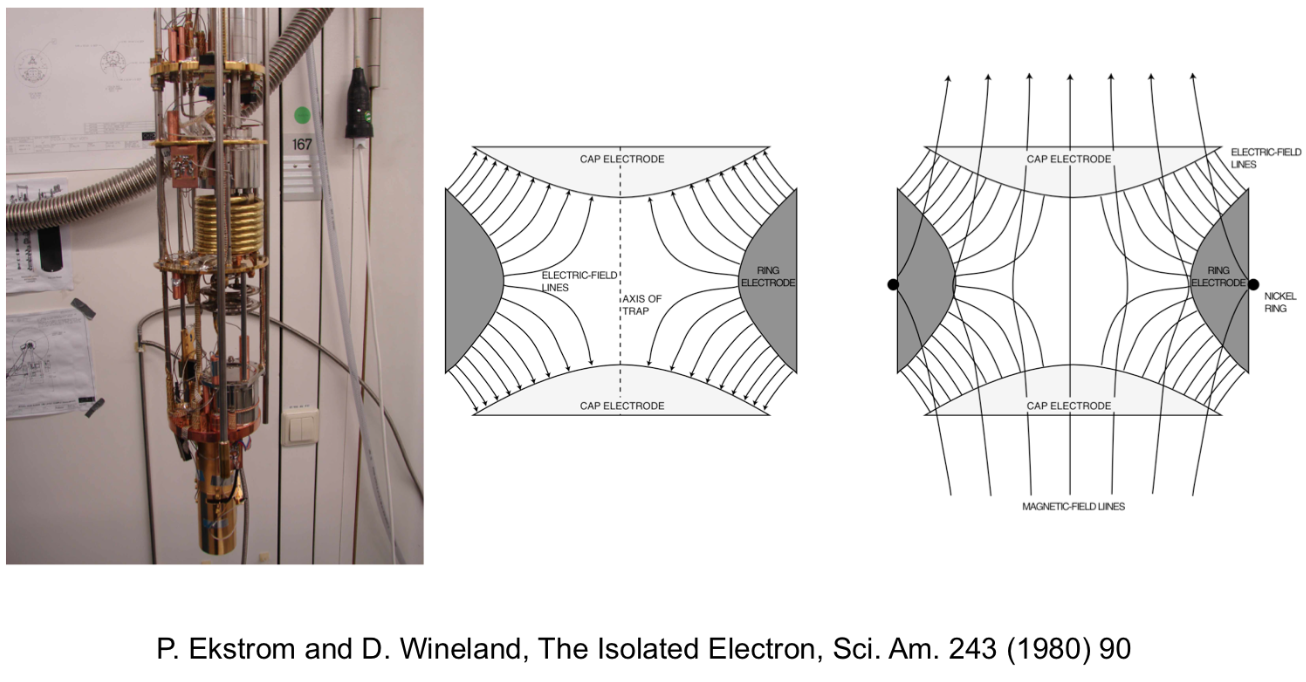
\includegraphics[scale=0.3]{penn_1.png}
\caption{Внешний вид и схема ловушки Пеннинга ~\cite{Courcera_NPh,Mart}}
\label{}
\end{figure}

Ядро стенда состоит из двух чашек электродов и ферромагнитного никелиевого кольца. Электрическая схема и модели измерения представлены на Рис.2 ~\cite{Courcera_NPh,Mart}\\

\begin{figure}[htp]
\centering
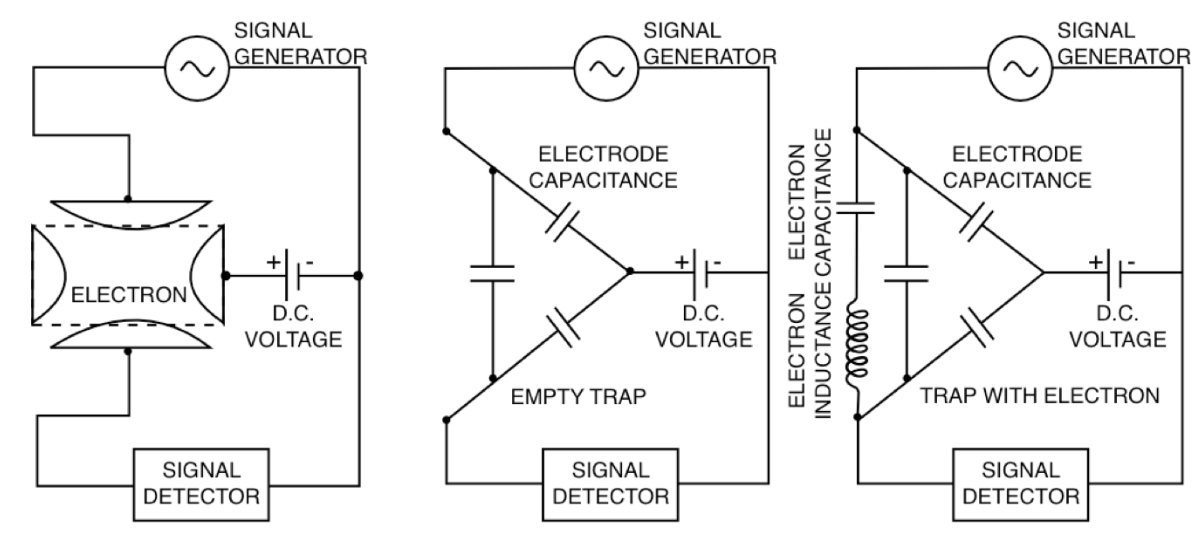
\includegraphics[scale=0.3]{penn_2.png}
\caption{Электрическая схема и модель измерений ~\cite{Courcera_NPh,Mart}}
\label{}
\end{figure}


\section{Принцип действия}
Принцип измерений приведен на Рис.2 \\

В пустой ловушке три электрода образуют емкостную сеть, которая передает сигнал переменного тока, генерируемый генератором. Захваченный электрон вносит в эту цепь дополнительную емкость-индуктивность. Таким образом, амплитуда передаваемого сигнала как функция частоты указывает количество электронов в устройстве и сдвиг частоты $\Delta \omega$ , из чего можно вычислить $g_e$ (13).

Результаты измерений приведены на Рис.3. \\
\begin{figure}[htp]
\centering
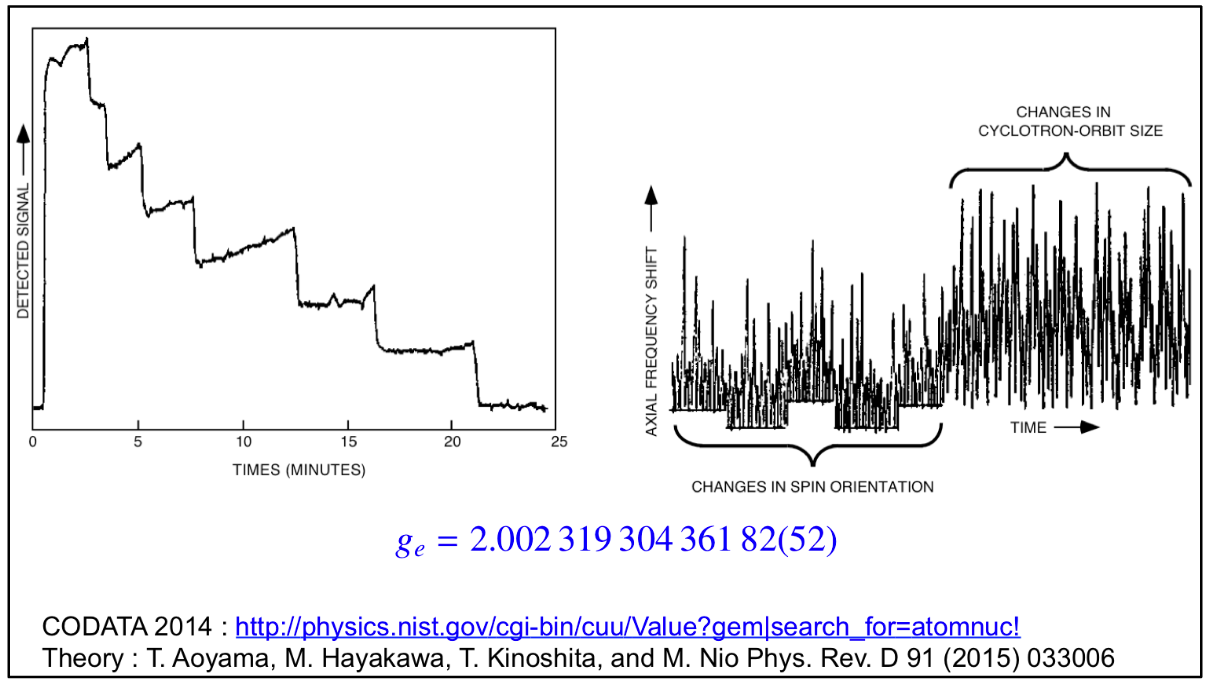
\includegraphics[scale=0.3]{penn_3.png}
\caption{Результаты измерений ~\cite{Courcera_NPh,Mart}}
\label{}
\end{figure}


\section{Рассчет движения электронов}
Рассчитаем движение электронов в ловушке ~\cite{Courcera_NPh}. Принебрежем незначительной неоднородностью магнитного поля, вызванное ферромагнитным никелиевым кольцом. \\

Пусть ось z сонаправлена вектору $\vec B$, тогда:
\begin{equation}
\vec B = \left(
\begin{array}{c}
0\\
0\\
B\\
\end{array}
\right)
\end{equation}

вектор потенциала:
\begin{equation}
\vec A = \left(
\begin{array}{c}
-B_y\\
0\\
0\\
\end{array}
\right)
\end{equation}

Гамильтониан такой системы с минимальной заменой:
\begin{equation}
H=\frac{1}{2m}(\vec p-e\vec A)^2 = 
\frac{1}{2m}(p^2 + 2e\vec p \vec A + e^2 A^2) =
 \frac{1}{2m}(p^2+2ep_xyB+e^2B^2y^2)
\end{equation}

Так как:
\begin{equation}
\omega = \frac{eB}{m}
\end{equation}
то, подставляя в (3) получим:
\begin{equation}
H=\frac{1}{2m}(p^2+2m\omega yp_x+m^2\omega^2 y^2)=\frac{1}{2m}(p_x^2+p_y^2+p_z^2) + \omega yp_x + \frac{m}{2}\omega^2 y^2
\end{equation}

Подставляем граничные условия
\begin{equation}
y_0 = \frac{p_x}{m\omega}
\end{equation}
в (5):
\begin{equation}
H = \frac{p_z^2}{2m} + \frac{p_y}{2m} + \frac{m\omega^2}{2}(y-y_0)^2
\end{equation}

Првое слагаемое $\frac{p_z^2}{2m}$ описывает движение электрона вдоль оси $z$, которое ограничено электродами. \\

Второе и третье слагаемое $\frac{p_y}{2m} + \frac{m\omega^2}{2}(y-y_0)^2$ описывают гармонические колебания электрона в экваториальной плоскости $xy$ \\

Энергетические уровни будут:
\begin{equation}
E = \omega(n+\frac{1}{2})
\end{equation}

Теперь учтем спин электрона в виде слагаемого:

\begin{equation}
\vec\mu_s\vec B
\end{equation}
, где: \\
$\vec\mu_s$ - вектор магнитного момента электрона; \\
$\vec B$ - вектор магнитного поля. \\

Тогда, Гамильтониан (7) запишется в виде:
\begin{equation}
H=\frac{1}{2m}(p_x^2+p_y^2+p_z^2) + \omega yp_x + \frac{m}{2}\omega^2 y^2 +\vec\mu_s\vec B
\end{equation}

Таким образом это даст дополнительное разделение на: 
\begin{equation}
 \pm g_e \frac{eB}{4m} = \pm \frac{g_e}{4}\omega
\end{equation}

И в итоге Гамильтониан будет:
\begin{equation}
H=\frac{1}{2m}(p_x^2+p_y^2+p_z^2) + \omega yp_x + \frac{m}{2}\omega^2 y^2 \pm \frac{g_e}{4}\omega
\end{equation}

Последний член в 4 раза больше той частоты, которую мы определили ранее. \\

Энергии $E_s$, соответствующие двум направлениям спина, будут отличаться от $E_n$ на $\pm \frac{g_e}{4}\omega$ \\


Таким образом, два направления спина $s_z=+\frac{1}{2},-\frac{1}{2}$ разделены той же разностью энергий $\omega$, что и основные уровни, при условии, что $g_e$ точно равно 2. Уровни энергии для сонаправленных и противоположно направленных оси $z$ спинов z смесятся на один шаг $\omega$. \\

Этого вырождения не было бы, если значение $g_e$ отличалось бы от 2, однако уровни все же слегка смещаются на частоту:

\begin{equation}
 \Delta\omega=\omega(g_e-2)/2
\end{equation}

, которую и можно измерить.\\

Характер движения электрона изображен на Рис.4\\

\begin{figure}[htp]
\centering
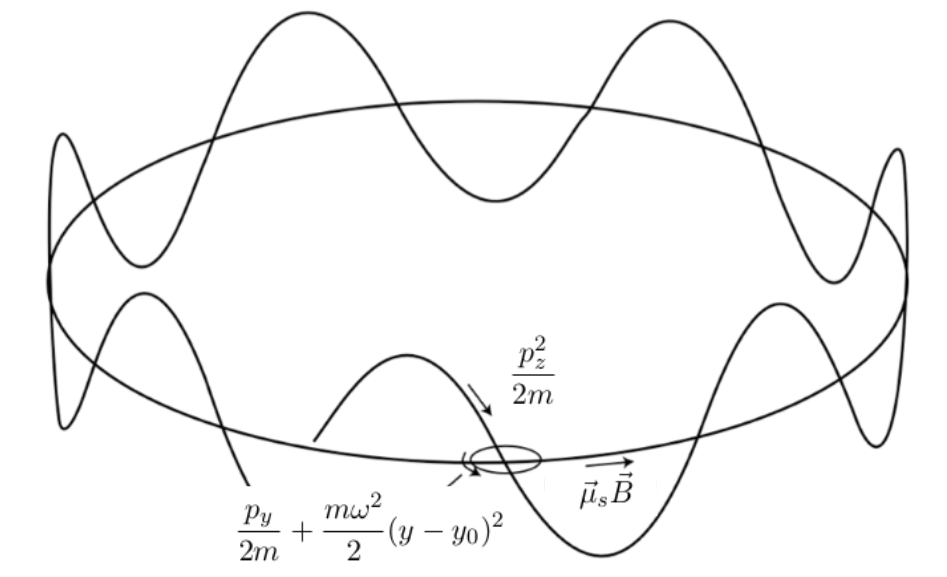
\includegraphics[scale=0.3]{penn_4.png}
\caption{Сложное движение электрона}
\label{}
\end{figure}

\section{Модернизация}
Для неразрушающего измерения спина, ранее рассмотренный стенд не подходит. В проекте ALPHA разработана модернизированная установка ~\cite{Alpha} \\
\begin{figure}[htp]
\centering
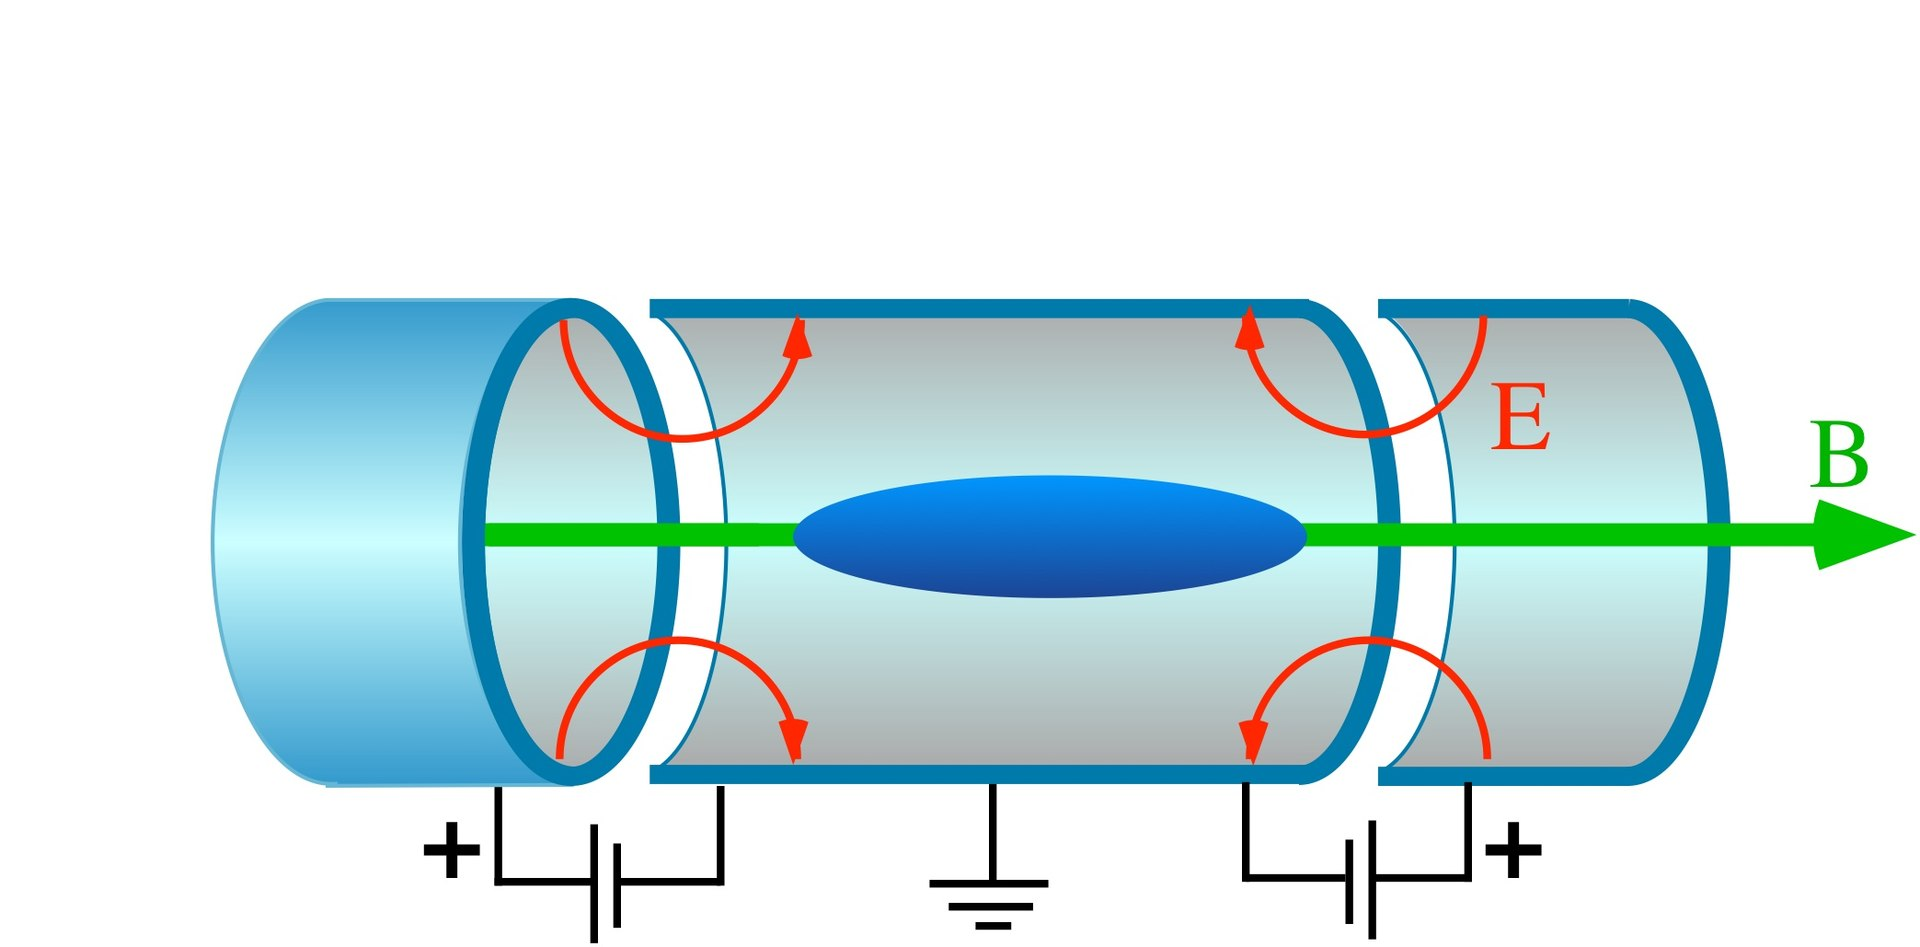
\includegraphics[scale=0.10]{Penning_Trap}
\caption{Внешний вид и схема ловушки Пеннинга ~\cite{Courcera_NPh,Mart}}
\label{}
\end{figure}

\section{Заключение}
Было продемонстрировано использование ловушки Пеннинга для измерения спина заряженных частиц для квантового компьютера. Видится перспективным создание лабораторного стенда ловушки Пеннинга на лабораторной базе Института ядерной энергетики и технической физики. Данный стенд может использоваться не только при исследовательских работах по квантовым вычислениям, но также и в лабораторном практикуме по ядерной физике: \\
измерении постоянной тонкой структуры ~\cite{Sarycheva}:

\begin{equation*}
\alpha = \frac{e^2}{4\pi\epsilon_0\hbar c} = \frac{1}{137}
\end{equation*}

измерении точного значения гиромагнитного отношения для электрона (до 14 знака) ~\cite{Mart}:
\begin{equation*}
g_e=\frac{\vec\mu}{\mu_B J} 
\end{equation*}
и других заряженных частиц.


\begin{thebibliography}{3}
\bibitem{Sysoev}
Сысоев С.С. Введение в квантовые вычисления. Квантовые алгоритмы, стр.35 -- СПб.: Издательство Санкт-Петербургского университета, 2020
\bibitem{Courcera_KvVich}
Сысоев С.С. Квантовые вычисления (Quantum computing) -- https://www.coursera.org/learn/kvantovyye-vychisleniya : Санкт-Петербургский государственный университет, 2020
\bibitem{Martin}
B.R.Martin, G.Shaw Particle physics, Third Edition, p.24 -- John Wilye and Sons Ltd, 2008
\bibitem{Courcera_NPh}
Martin Pohl, Anna Sfyrla, Mercedes Paniccia Particle Physics: an Introduction., 4.2 Electromagnetic scattering -- https://www.coursera.org/learn/particle-physics/lecture/Vd0tP/4-2-electromagnetic-scattering Университет Женевы, 2020
\bibitem{Sarycheva}
Л.И.Сарычева Введение в физику микромира. Физика частиц и ядер. стр.17 -- М.: Книжный дом <<ЛИБРОКОМ>>, 2012 
\bibitem{Mart}
Martin Pohl Particles, Fields, Space-Time: From Thomson's Electron to Higgs' Boson -- CRC Press, 2020
\bibitem{Ekstrom}
P.Ekstrom and D.Wineland The Isolated Electorn -- Scientific American, 243, p.90 -- 1980
\bibitem{Giancoli}
Douglas C.Giancoli Physics for Scientists and Engineers with Modern Physics, Fourth Edition, p.1301 -- England: Pearson Education Limited, 2014 
\bibitem{wiki}
Ловушка Пеннинга -- \url{https://en.wikipedia.org/wiki/Penning_trap}
\bibitem{Alpha}
Проект ALPHA -- \url{https://alpha.web.cern.ch/penning-trap }
\end{thebibliography}

\end{document}

